\section{Evaluation}
\label{chapter:evaluation}

This chapter discusses the evaluation criteria with dataset simulation as well as 
the issues and solutions on social and ethical aspects appears with this system design.
Surely, our system still has limitations, 
we then discusse the most important two limitations within our system: 
evaluation outdated and game playability.

\subsection{Success Criterias}

\subsubsection{Model Evaluation by Simulation}

In the previous chapter of design and model, we descrived the system data flow, which is
done by three main step: task generation, malicious player detection and disaster level evaluation as well.
The second step malicious player detection is essentially a classification problem that 
our system detect the new player is reliable or not based on \hyperref[def:tv]{Trust Value}.

To evaluate our model, a typical classification model performance evaluation metric is to 
using the Receiver Operating Characteristic (ROC) curve \cite{hanley1982meaning}, which 
plots True Positive (on the y-axis) against False Positive and the ideal \textbf{surface under the ROC curve} is 1.
Nevertheless, before we test the system with real user, one can generate a reaonsable random dataset 
to test the performance of our classification model (\hyperref[idx:prm]{PRM}).

Our player have two different type of inputs: \textbf{the \hyperref[def:roi]{ROI}, 
and its \hyperref[def:tagv]{Tag Vector}}. For a reaonsable player data entity, 
one has to define the ROI selection and its corresponding Tag Vector.
To generate resonable ROI to simulate real user behavior, we disscuss the click behavior
of a desktop target click behavior first.

The target click behavior has been researched for years and address by FFitts Law \cite{bi2013ffitts}.
It modeled and proved the distribution of click behavior for a certain click goal point is a Gaussian distribution \cite{goodman1963statistical}.
Thus, with frequency statistic view, the actual ROI(s) for a certain exists, 
and whatever the user start from the top right corner or bottom left corner or etc., 
according to the FFitts Law, the starting click point should follows normal distribution around the actual point,
as shown in figure \ref{fig:evaluation}. Similarly, the landing point of the selection of ROI(s)
should also follows a normal distribution. 

\begin{figure}[htp]
\centering
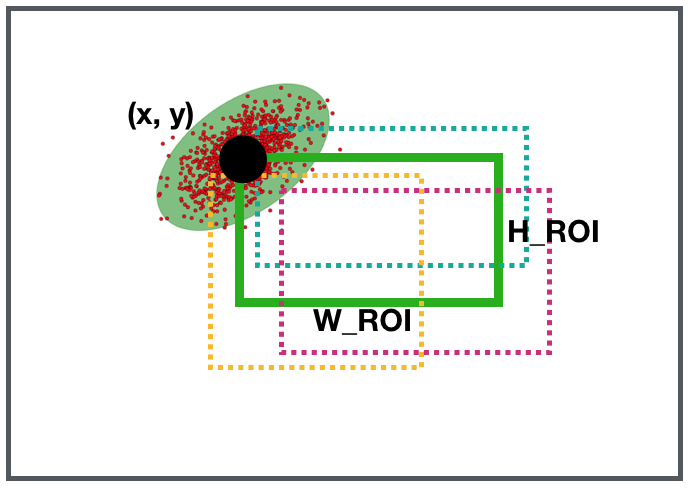
\includegraphics[width=0.5\columnwidth]{figures/evaluation}
\caption{Example of ROI Simulation}
\label{fig:evaluation}
\end{figure}

Therefore, to generate ROI(s), let $(x, y)$ is the player ROI starting point, $(H_{ROI}$, $W_{ROI})$ is the height
and width pair of this ROI, then we generate noise for the ROI starting points and landing points: 
$(x+\epsilon, y+\epsilon), (H_{ROI}+\epsilon, W_{ROI}+\epsilon)$ and $\epsilon \sim N(0, \delta)$.
For the paremeter $\delta$, one can use Maximum Likelihood estimator \cite{johansen1990maximum} 
to perform the inference from all manually ROI selection samples from initial trusted group.

The generation of Tag Vector for a certain image is much simple than ROI's, 
a randomly pick from initial trusted group is sufficient for the simulation case 
because these tags are trusted results and a partial randomly selection already introduced the noise in this case.

Eventually, one can perform this random dataset on the system to evaluate \textbf{surface under the ROC curve} to
evaluate the overall performance of this system (the model shows good performance if the surface approximate to 1), 
which gives the theoretical evaluation results.

\subsubsection{Issues on Social and Ethical Aspects}
\label{chapter:ethical}

\textbf{Intellectual Property Rights:} 
Our disaster monitoring system is an non-commercial project which invites volunteers to contribute to it. 
It is used to help the UNICEF and other non-profit organizations deliver supplies in disaster areas safer. 
So the IPR on the annotations should not belong to the volunteer users. In an appropriate manner, user will be informed that 
his or her contribution to the system is volunteering and the produced data will be used only for 
monitoring disasters in Syria.

\textbf{Leakage of data:} 
Malicious issues are not limited to the spite of game playing but also possible on the issue of leakage of our image data.
Malicious players also can be terrorists, they can use these satellite image as a free attack resources 
if we provide the entire region image to the game player, which leads to the data insecurity.
Therefore, we cut big satellite image into small segmentations in our system to prevent data leakage to ordinary players
for the data security reason.

\textbf{Information Loss}
We cut big region images into small fragements areas to prevent leakage of data. 
However this method will cause some information loss problem if some important ROIs are 
located at the intersection of two dividing lines.
A possible solution for this limitation is to consider ``Half Shifting'' cut. 
The ``Half Shifting'' cut have two grids, 
the one obtained from the other shift the original grid to the right and to the bottom by half the breath 
respectively hight of a ROI, as shown in figure \ref{fig:information_loss}. Note that this solution that
only increases the number of region pictures, it does not influence any model and system design.

\begin{figure}[H]
\centering
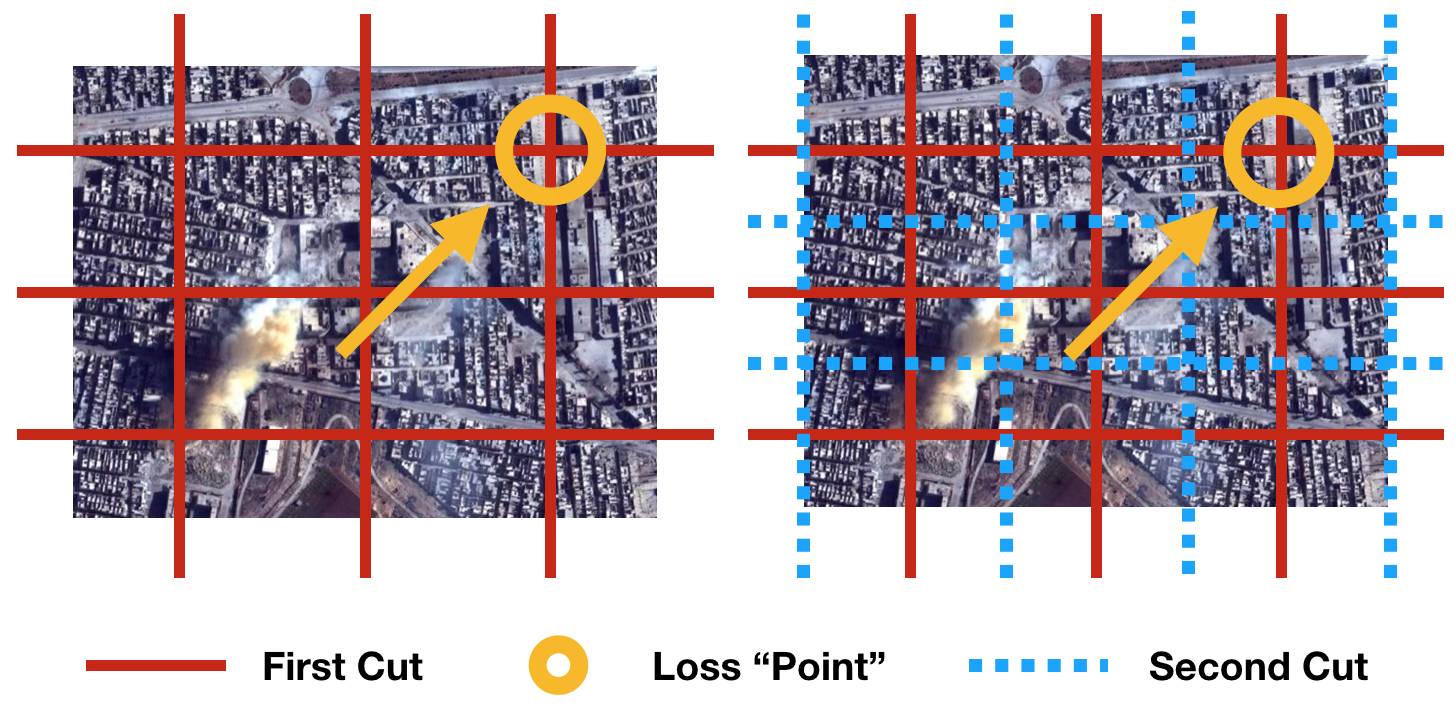
\includegraphics[width=0.7\columnwidth]{figures/information_loss3}
\caption{
    \textbf{Information Loss}: Information loss may occurs on the intersection lines, as shown on the left; 
    a possible solution is to perform a ``Half Shifting'' cut
}
\label{fig:information_loss}
\end{figure}

\subsection{Limitations of the System}

\subsubsection{Evaluation Outdated}

A limitation occurs in a situation that our \hyperref[idx:prg]{PRG} network is based on image dependent prespective, that leads,
each calculated \hyperref[def:dl]{Disaster Level} get invalid if the region image is outdated.
We assume the satellite machine monitors an region and take pictures between intervals. 
However, our evaluation the model only calculate the disaster level at a unique moment, 
which means the disaster level need transvaluation when a new image comes out.
If none of all the new images from a region get evaluate, then the disaster level will not be calculated.

Note that the disaster level of a disaster region over time is essentially a non-stationary process \cite{brockwell2013time} 
due to the paroxysmal disaster situation. One can directly perform time series prediction method \cite{kuznetsov2015learning}
on the disaster level time series. 
Unfortunately, there is no space to cover them in depth.

\subsubsection{Gameplay and Playability}

The GWAP collects satellite photos of disaster areas. But even if in the disaster areas, 
not every part of the areas has a disaster. Most parts of the earth are lake, forest, 
desert and so on, which means the users may meet the situation that there is no available 
ROI in several continuous rounds. Obviously, it will decrease the playability and enjoyment of the game.
Our system is just a very simple tagging game at present, users can not get enough enjoyment they want in it. 
And it is too reliant on the unpaid volunteers to donate their time to contribute information. 
We should make the system more interesting and appealing in the future work.